\documentclass[a4paper, table]{article}
% Useful packages, sorted so packages of similar functionality are grouped together. Not all are essential to make the document work, however an effort was made to make this list as minimalistic as possible. Feel free to add your own!

% Essential for making this template work are graphicx, float, tabularx, tabu, tocbibind, titlesec, fancyhdr, xcolor and tikz. 

% Not essential, but you will have to debug the document a little bit when removing them are amsmath, amsthm, amssymb, amsfonts, caption, subcaption, appendix, enumitem, hyperref and cleveref.

% inputenc, lipsum, booktabs, geometry and microtype are not required, but nice to have.

\usepackage[portuguese]{babel} % Set document language
\usepackage[utf8]{inputenc} % Allows the use of some special characters
\usepackage{textcomp} % Allows the use of Text Companion fonts

\usepackage{amsmath, amsthm, amssymb, amsfonts} % Nicer mathematical typesetting
\usepackage{biblatex} % Imports biblatex package
\usepackage{listings} % Allows to highlight code

\usepackage{graphicx} % Allows the use of \begin{figure} and \includegraphics
\usepackage{float} % Useful for specifying the location of a figure ([H] for ex.)
\usepackage{caption} % Adds additional customization for (figure) captions
\usepackage{subcaption} % Needed to create sub-figures

\usepackage{tabularx} % Adds additional customization for tables
\usepackage{tabu} % Adds additional customization for tables
\usepackage{booktabs} % For generally nicer looking tables

\usepackage[margin = 2.5cm]{geometry} % Allows for custom (wider) margins
\usepackage{microtype} % Slightly loosens margin restrictions for nicer spacing  
\usepackage{titlesec} % Used to create custom section and subsection titles
\usepackage{titletoc} % Used to create a custom ToC
\usepackage{appendix} % Any chapter after \appendix is given a letter as index
\usepackage{fancyhdr} % Adds customization for headers and footers
\usepackage[shortlabels]{enumitem} % Adds additional customization for itemize
% \usepackage{setspace} % Allows custom spacing of the lines

\usepackage{hyperref} % Allows links and makes references and the ToC clickable
\usepackage[noabbrev, capitalise]{cleveref} % Easier referencing using \cref{<label>} instead of \ref{}

\usepackage{xcolor} % Predefines additional colors and allows user defined colors

\usepackage{tikz} % Useful for drawing images, used for creating the frontpage
\usetikzlibrary{positioning} % Additional library for relative positioning 
\usetikzlibrary{calc} % Additional library for calculating within tikz

% Defines a command used by tikz to calculate some coordinates for the front-page
\makeatletter
\newcommand{\gettikzxy}[3]{%
  \tikz@scan@one@point\pgfutil@firstofone#1\relax
  \edef#2{\the\pgf@x}%
  \edef#3{\the\pgf@y}%
}
\makeatother
 % Loads in the preamble 
% Give your report a title
\newcommand\reporttitle{
    Tutoorial API RESTful com Fastify e Mongoose
}

% Insert course code, name, quartile number and year (or any other subtitle)
\newcommand\reportsubtitle{
    MES, Sistemas de Informação para a Internet - 2022
}

% Add your group number or any other text.
\newcommand\groupnumber{
    \textbf{Grupo}
}

% Insert authors and student numbers here
\newcommand\reportauthors{
    Edgar Santos & 201600264 \\
}

% Add the name of your tutor or any other text.
\newcommand\grouptutor{
    Professor: José Pereira
}

% Date and location (default: current date and Eindhoven)
\newcommand\placeanddate{
    Setúbal, \today
}

% Set caption label for listings
\renewcommand{\lstlistingname}{Código}

% Define Ips-orange (color of the TU/e logo). Can be changed to drastically change the look of the template
\definecolor{Ips-orange}{RGB}{241, 135, 53}

% Import the bibliography file
\addbibresource{General/References.bib}

% Force all bibliography entries to display even when no cited in the text
\nocite{*}

% All of the following code can be removed to be left with (close to) default LaTeX behaviour. 

% Sets up hyperlinks in the document to be colored
\hypersetup{
    colorlinks=true,
    linkcolor=Ips-orange,
    urlcolor=Ips-orange,
    citecolor=Ips-orange
}
\urlstyle{same} % Defines settings for link and reference formatting

% Change bullet style for level 1, 2 and 3 respectively for itemize
\renewcommand{\labelitemi}{\scriptsize\textcolor{Ips-orange}{$\blacksquare$}}% level 1
\renewcommand{\labelitemii}{\scriptsize\textcolor{Ips-orange}{$\square$}}% level 2
\renewcommand{\labelitemiii}{\textcolor{Ips-orange}{$\circ$}}% level 3

% \renewcommand{\labelitemi}{\small\textcolor{Ips-orange}{\ding{70}}} % level 1
% \renewcommand{\labelitemii}{\small\textcolor{Ips-orange}{\ding{71}}}% level 2
% \renewcommand{\labelitemiii}{\tiny\textcolor{Ips-orange}{\ding{71}}}% level 3

% Change bullet style for level 1, 2 and 3 respectively for enumerate
\renewcommand{\labelenumi}{\textbf{\textcolor{Ips-orange}{\arabic*.}}}% level 1
\renewcommand{\labelenumii}{\textbf{\textcolor{Ips-orange}{[\alph*]}}}% level 2
\renewcommand{\labelenumiii}{\textbf{\textcolor{Ips-orange}{\roman*.}}}% level 3

% Have reference labels be linked to section (section 3 will have fig. 3.1 etc.)
\counterwithin{equation}{section} % For equations
\counterwithin{figure}{section} % For figures
\counterwithin{table}{section} % For tables

% Increase head height and compensate top margin
\setlength{\headheight}{24pt}
\addtolength{\topmargin}{-4pt}

% Creates a beautiful header/footer
\pagestyle{fancy}
\lhead{
\includegraphics[height = 16pt]{Figures/0. General/ips_logo_small.pdf}}
\rhead{\reporttitle}
\renewcommand{\footrulewidth}{0.4pt}
\cfoot{Página \thepage}

% Formats section, subsection and subsubsection titles respectively 
\titleformat{\section}{\sffamily\color{Ips-orange}\Large\bfseries}{\thesection\enskip\color{gray}\textbar\enskip}{0cm}{} % Formats section titles

\titleformat{\subsection}{\sffamily\color{Ips-orange}\large\bfseries}{\thesubsection\enskip\color{gray}\textbar\enskip}{0cm}{} % Formats subsection titles

\titleformat{\subsubsection}{\sffamily\color{Ips-orange}\bfseries}{\thesubsubsection\enskip\color{gray}\textbar\enskip}{0cm}{} % Formats subsubsection titles

% Formats captions
\DeclareCaptionFont{Ips-orange}{\color{Ips-orange}}
\captionsetup{labelfont={Ips-orange,bf}}

% Changes font to mlmodern
\usepackage{mlmodern}

% Adds spacing between paragraphs
\setlength\parskip{6pt}

% Removes indent when starting a new paragraph
\setlength\parindent{0pt}

% Makes the text of the whole document one-and-a-half spaced. Footnotes, figures, and tables will still be singlespaced, however.
% \onehalfspacing

% Limits the ToC to sections and subsections (no subsubsec.)
% \setcounter{tocdepth}{2}

% Define additional required colors
\definecolor{gray}{rgb}{0.5, 0.5, 0.5}
\definecolor{mediumgray}{rgb}{0.3, 0.4, 0.4}
\definecolor{mediumblue}{rgb}{0.0, 0.0, 0.8}
\definecolor{forestgreen}{rgb}{0.13, 0.55, 0.13}
\definecolor{darkviolet}{rgb}{0.58, 0.0, 0.83}
\definecolor{royalblue}{rgb}{0.25, 0.41, 0.88}
\definecolor{crimson}{rgb}{0.86, 0.8, 0.24}
\colorlet{punct}{red!60!black}
\definecolor{background}{HTML}{EEEEEE}
\definecolor{delim}{RGB}{20,105,176}
\colorlet{numb}{magenta!60!black}

% Formats code highlight
\lstset{
    backgroundcolor=\color{background},         % choose the background color. You must add \usepackage{color}
    basicstyle=\footnotesize\ttfamily,          % the font basic style that is used for the code
    breakatwhitespace=false,                    % sets if automatic breaks should only happen at whitespace
    breaklines=true,                            % sets automatic line breaking
    captionpos=b,
    columns=fullflexible,
    commentstyle=\color{mediumgray}\upshape,    % comment style
    emph={},
    emphstyle=\color{crimson},
    extendedchars=true,                         % requires inputenc
    fontadjust=true,
    frame=lines,                               % adds a frame around the code
    identifierstyle=\color{black},
    keepspaces=true,
    keywordstyle=\color{mediumblue},            % keyword style
    keywordstyle={[2]\color{darkviolet}},
    keywordstyle={[3]\color{royalblue}},
    numbers=left,                               % where to put the line-numbers
    numbersep=5pt,                              % how far the line-numbers are from the code
    numberstyle=\tiny\color{gray},        % the style that is used for the line-numbers
    stepnumber=1,                               % the step between two line-numbers. If it's 1, each line will be numbered
    rulecolor=\color{black},                    % if not set, the frame-color may be changed on line-breaks within not-black text (e.g. commens (green here))
    showlines=true,
    showspaces=false,
    showstringspaces=false,                     % underline spaces within strings
    showtabs=false,                             % show tabs within strings adding particular underscores
    stringstyle=\color{forestgreen},            % string literal style
    tabsize=2,                                  % sets default tab size to 2 spaces
    title=\lstname,                             % show the filename of files included with \lstinputlisting;
    upquote=true,                               % requires textcomp
}

% Fix listings issues with most characters in latin languages
\lstset{literate=
    {á}{{\'a}}1 {é}{{\'e}}1 {í}{{\'i}}1 {ó}{{\'o}}1 {ú}{{\'u}}1
{Á}{{\'A}}1 {É}{{\'E}}1 {Í}{{\'I}}1 {Ó}{{\'O}}1 {Ú}{{\'U}}1
{à}{{\`a}}1 {è}{{\`e}}1 {ì}{{\`i}}1 {ò}{{\`o}}1 {ù}{{\`u}}1
{À}{{\`A}}1 {È}{{\'E}}1 {Ì}{{\`I}}1 {Ò}{{\`O}}1 {Ù}{{\`U}}1
{ä}{{\"a}}1 {ë}{{\"e}}1 {ï}{{\"i}}1 {ö}{{\"o}}1 {ü}{{\"u}}1
{Ä}{{\"A}}1 {Ë}{{\"E}}1 {Ï}{{\"I}}1 {Ö}{{\"O}}1 {Ü}{{\"U}}1
{â}{{\^a}}1 {ê}{{\^e}}1 {î}{{\^i}}1 {ô}{{\^o}}1 {û}{{\^u}}1
{Â}{{\^A}}1 {Ê}{{\^E}}1 {Î}{{\^I}}1 {Ô}{{\^O}}1 {Û}{{\^U}}1
{ã}{{\~a}}1 {ẽ}{{\~e}}1 {ĩ}{{\~i}}1 {õ}{{\~o}}1 {ũ}{{\~u}}1
{Ã}{{\~A}}1 {Ẽ}{{\~E}}1 {Ĩ}{{\~I}}1 {Õ}{{\~O}}1 {Ũ}{{\~U}}1
{œ}{{\oe}}1 {Œ}{{\OE}}1 {æ}{{\ae}}1 {Æ}{{\AE}}1 {ß}{{\ss}}1
{ű}{{\H{u}}}1 {Ű}{{\H{U}}}1 {ő}{{\H{o}}}1 {Ő}{{\H{O}}}1
{ç}{{\c c}}1 {Ç}{{\c C}}1 {ø}{{\o}}1 {å}{{\r a}}1 {Å}{{\r A}}1
{€}{{\euro}}1 {£}{{\pounds}}1 {«}{{\guillemotleft}}1
{»}{{\guillemotright}}1 {ñ}{{\~n}}1 {Ñ}{{\~N}}1 {¿}{{?`}}1 {¡}{{!`}}1
}

% Add JavaScript language support to listings
\lstdefinelanguage{JavaScript}{
    morekeywords=[1]{break, continue, delete, else, for, function, if, in,
            new, return, this, typeof, var, void, while, with},
    % Literals, primitive types, and reference types.
    morekeywords=[2]{false, null, true, boolean, number, undefined,
            Array, Boolean, Date, Math, Number, String, Object},
    % Built-ins.
    morekeywords=[3]{eval, parseInt, parseFloat, escape, unescape},
    sensitive,
    morecomment=[s]{/*}{*/},
    morecomment=[l]//,
    morecomment=[s]{/**}{*/}, % JavaDoc style comments
    morestring=[b]',
    morestring=[b]"
}[keywords, comments, strings]

\lstdefinelanguage[ECMAScript2015]{JavaScript}[]{JavaScript}{
    morekeywords=[1]{await, async, case, catch, class, const, default, do,
            enum, export, extends, finally, from, implements, import, instanceof,
            let, static, super, switch, throw, try},
    morestring=[b]` % Interpolation strings.
}
\lstalias[]{ES6}[ECMAScript2015]{JavaScript}

% Add JSON language support to listings
\lstdefinelanguage{JSON}{
literate=
*{0}{{{\color{numb}0}}}{1}
{1}{{{\color{numb}1}}}{1}
{2}{{{\color{numb}2}}}{1}
{3}{{{\color{numb}3}}}{1}
{4}{{{\color{numb}4}}}{1}
{5}{{{\color{numb}5}}}{1}
{6}{{{\color{numb}6}}}{1}
{7}{{{\color{numb}7}}}{1}
{8}{{{\color{numb}8}}}{1}
{9}{{{\color{numb}9}}}{1}
{:}{{{\color{punct}{:}}}}{1}
{,}{{{\color{punct}{,}}}}{1}
{\{}{{{\color{delim}{\{}}}}{1}
{\}}{{{\color{delim}{\}}}}}{1}
{[}{{{\color{delim}{[}}}}{1}
{]}{{{\color{delim}{]}}}}{1},
}
 % Loads in user defined settings
\begin{document}

% Inserts the front page
\begin{titlepage}

    \centering

    % Advanced header
    % \begin{tikzpicture}

    %     \node[opacity=0.3,inner sep=0pt,remember picture,overlay] at (4.5,-0.5){\includegraphics[width= 0.8 \textwidth]{Figures/0. General/tue_logo_gray.pdf}};

    %     \node[inner sep=0pt] (logo) at (0,0)
    %     {
\includegraphics[width=.25\textwidth]{Figures/0. General/ips_logo_small.pdf}};

    %     \node[text width = 0.5\textwidth, right = of logo, execute at begin node=\setlength{\baselineskip}{5ex}](title){\sffamily\huge\reporttitle};

    %     \node[text width = 0.5\textwidth, yshift = 0.75cm, below = of title](subtitle){\sffamily\Large\reportsubtitle};

    %     \gettikzxy{(subtitle.south)}{\sffamily\subtitlex}{\subtitley}
    %     \gettikzxy{(title.north)}{\titlex}{\titley}
    %     \draw[line width=1mm, Ips-orange]($(logo.east)!0.5!(title.west)$) +(0,\subtitley) -- +(0,\titley);

    % \end{tikzpicture}

    \tikz \node[inner sep = 0pt] at (0,0) {
\includegraphics[width = 0.6\textwidth]{Figures/0. General/ips_logo.pdf}};

    \vspace{5cm}

    \sffamily \huge \reporttitle

    \vspace{0.5cm}

    \sffamily \Large \reportsubtitle

    \vspace{3cm}

    \sffamily \normalsize \groupnumber

    \begin{table}[H]
        \centering
        \sffamily
        \large
        \begin{tabu} to 0.8\linewidth {cc}
            \textbf{Nome} & \textbf{Número de Estudante} \\
            \hline

            \sffamily\reportauthors
        \end{tabu}

    \end{table}

    \sffamily \normalsize \grouptutor

    % Footer image
    % \tikz[remember picture,overlay]\node[anchor=south,inner sep=0pt] at (current page.south) {\includegraphics[width=\paperwidth]{Figures/0. General/tue.pdf}};

    \vfill

    \sffamily \Large {\placeanddate} \\

\end{titlepage}









\newpage

% Generates a ToC without page number
{\hypersetup{linkcolor=black} % Keeps the ToC black even with non-black link color
    \tableofcontents\thispagestyle{empty}}
\newpage

% contains inspiration for formatting tables, images, text citations etc.
% \pagenumbering{roman}

\section{This is a section}
\subsection{This is a subsection}

\subsubsection{This is a subsubsection}
This section contains some templates that can be used to create a uniform style within the document. It also shows of the overall formatting of the template, created using the predefined styles from the \texttt{settings.tex} file.

\subsection{General formatting}
Firstly, the document uses the font mlmodern, using no indent for new paragraphs and commonly uses the color \textcolor{Ips-orange}{Ips-orange} (the color of the TU/e logo) in its formatting. It uses the \texttt{fancyhdr} package for its headers and footers, using the TU/e logo and report title as the header and the page number as the footer. The template uses custom section, subsection and subsubsection formatting making use of the \texttt{titlesec} package.\\
The \texttt{hyperref} package is responsible for highlighting and formatting references like figures and tables. For example \cref{table: style 1} or \cref{fig: three images}. It also works for citations \cite{texbook}. Note how figure numbers are numbered according to the format \texttt{<chapter number>.<figure number>}.\\

Bullet lists are also changed globally, for a maximum of 3 levels:

\begin{itemize}
    \item Item 1
    \item Item 2
          \begin{itemize}
              \item subitem 1
                    \begin{itemize}
                        \item subsubitem 1
                        \item subsubitem 2
                    \end{itemize}
          \end{itemize}
    \item Item 3
\end{itemize}

Similarly numbered lists are also changed document wide:

\begin{enumerate}
    \item Item 1
    \item Item 2
          \begin{enumerate}
              \item subitem 1
                    \begin{enumerate}
                        \item subsubitem 1
                        \item subsubitem 2
                    \end{enumerate}
          \end{enumerate}
    \item Item 3
\end{enumerate}

\newpage

\subsection{Tables and figures}
The following table, \cref{table: style 1}, shows a possible format for tables in this document. Alternatively, one can also use the black and white version of this, shown in \cref{table: style 2}. Note that caption labels are in the format \textbf{\textcolor{Ips-orange}{Table x.y:} }
\begin{table}[ht]
    \rowcolors{2}{Ips-orange!10}{white}
    \centering
    \caption{A table without vertical lines.}
    \begin{tabular}[t]{ccccc}
        \toprule
        \color{Ips-orange}\textbf{Column 1} & \color{Ips-orange}\textbf{Column 2} & \color{Ips-orange}\textbf{Column 3} & \color{Ips-orange}\textbf{Column 4} & \color{Ips-orange}\textbf{Column 5} \\
        \midrule
        Entry 1                             & 1                                   & 2                                   & 3                                   & 4                                   \\
        Entry 2                             & 1                                   & 2                                   & 3                                   & 4                                   \\
        Entry 3                             & 1                                   & 2                                   & 3                                   & 4                                   \\
        Entry 4                             & 1                                   & 2                                   & 3                                   & 4                                   \\
        \bottomrule
    \end{tabular}
    \label{table: style 1}
\end{table}

\begin{table}[ht]
    \rowcolors{2}{gray!10}{white}
    \centering
    \caption{A table without vertical lines.}
    \begin{tabular}[t]{ccccc}
        \toprule
        \textbf{Column 1} & \textbf{Column 2} & \textbf{Column 3} & \textbf{Column 4} & \textbf{Column 5} \\
        \midrule
        Entry 1           & 1                 & 2                 & 3                 & 4                 \\
        Entry 2           & 1                 & 2                 & 3                 & 4                 \\
        Entry 3           & 1                 & 2                 & 3                 & 4                 \\
        Entry 4           & 1                 & 2                 & 3                 & 4                 \\
        \bottomrule
    \end{tabular}
    \label{table: style 2}
\end{table}

For normal, single image figures, the standard \texttt{\textbackslash begin\{figure\}} environment can be used. For multi-image figures, one could use either the \texttt{\textbackslash begin\{subfigure\}} environment to get a main caption with 3 subcaptions like \cref{fig: three images} or the \texttt{\textbackslash begin\{minipage\}} environment to get 3 independent captions like \cref{fig: style 2 image a} - \ref{fig: style 2 image c}

\begin{figure}[H]
    \centering
    \begin{subfigure}[b]{0.3\textwidth}
        \centering
        \includegraphics[width=\textwidth]{example-image-a}
        \caption{image a}
        \label{fig: style 1 image a}
    \end{subfigure}
    \hfill
    \begin{subfigure}[b]{0.3\textwidth}
        \centering
        \includegraphics[width=\textwidth]{example-image-b}
        \caption{image b}
        \label{fig: style 1 image b}
    \end{subfigure}
    \hfill
    \begin{subfigure}[b]{0.3\textwidth}
        \centering
        \includegraphics[width=\textwidth]{example-image-c}
        \caption{image c}
        \label{fig: style 1 image c}
    \end{subfigure}
    \caption{Three images}
    \label{fig: three images}
\end{figure}

\begin{figure}[H]
    \centering
    \begin{minipage}{0.3\textwidth}
        \centering
        \includegraphics[width=\textwidth]{example-image-a}
        \captionof{figure}{image a}
        \label{fig: style 2 image a}
    \end{minipage}
    \hfill
    \begin{minipage}{0.3\textwidth}
        \centering
        \includegraphics[width=\textwidth]{example-image-b}
        \captionof{figure}{image b}
        \label{fig: style 2 image b}
    \end{minipage}
    \hfill
    \begin{minipage}{0.3\textwidth}
        \centering
        \includegraphics[width=\textwidth]{example-image-c}
        \captionof{figure}{image c}
        \label{fig: style 2 image c}
    \end{minipage}
\end{figure}

\newpage

\subsection{Code}

\lstinputlisting[language=XML, caption=Example File]{Listings/Z. Template/Example.xml} % Feel free to remove / comment out
% \newpage

% Starting page numbering
\pagenumbering{arabic}

% Creates the introduction
\section{Introdução} \label{section: introduction}

Neste tutorial vamos construir uma aplicação simples para gerir os produtos da ementa de um restaurante. O foco estará no desenvolvimento de uma solução backend em Node.js \cite{nodejs_nodejs_nodate} utilizando a \textit{framework} \textbf{fastify} \cite{noauthor_fastify_nodate} para a criação das rotas responsáveis por gerir todas as operações CRUD \cite{noauthor_what_nodate} dos nossos produtos. A nível de persistência será utilizada a biblioteca \textbf{mongoose} \cite{noauthor_mongoose_nodate} para simplificar a modelação de objetos de uma base de dados MongoDB \cite{noauthor_mongodb_nodate}.

\subsection{Pré-requisitos}

Para tirar o máximo partido deste tutorial, deverá compreender o fundamental dos princípios REST \cite{noauthor_what_nodate-1}, bem como conhecer o básico de MongoDB e de uma \textit{framework} web de Node.js, como o Express.js \cite{noauthor_express_nodate}.

Será utilizada a sintaxe do ES6 \cite{noauthor_ecmascript_nodate}, pelo qual se espera o conhecimento de conceitos como desestruturação, funções \textit{arrow} e outros. De qualquer modo, todo o código o apresentado será explicado em detalhe.

De modo geral, os princípios demonstrados neste projeto não são particularmente complexos, pelo que este tutorial pode ser considerado como uma introdução às tecnologias listadas acima.

\newpage

% Creates the tutorial chapter
\section{Tutorial} \label{section: tutorial}

\subsection{Preparando o Projeto} \label{section: tutorial project setup}

Assegure-se de que tem o Node.js instalado globalmente na sua máquina antes de começarmos; isto permitir-nos-á importar todas as nossas dependências e inicializar o projeto. Além disso, para a base de dados será utilizada uma \textit{cluster} gratuito hospedado no MongoDB Atlas \cite{noauthor_mongodb_nodate-1}, mas poderá, em alternativa, utilizar uma instância local do MongoDB.

Vamos começar por criar uma nova pasta para o projeto, instalar as nossas dependências, e montar a estrutura. No terminal do seu computador execute o seguinte:

\lstinputlisting[language=SH, caption=Comandos para a inicialização do projeto]{Listings/1. Tutorial/project_setup.sh}

Então, linha por linha: (1) criámos a pasta \texttt{api-ementa}, (2) entramos na pasta criada, (3) inicializámos um projeto Node, (4) instalámos o Fastify e o Mongoose como dependências, (5)criámos uma nova pasta \texttt{src} com (6) um ficheiro \texttt{index.js} que será a raiz da nossa aplicação.

\subsubsection{Inicializando o Fastify e Mongoose}

Em seguida, vamos fazer a nossa aplicação Fastify funcionar com a ligação ao MongoDB.

Portanto, no ficheiro \texttt{index.js} que acabamos de criar vamos colocar o seguinte:

\lstinputlisting[language=ES6, caption=Ficheiro index.js inicial]{Listings/1. Tutorial/index_1.js}

Começamos por importar o \texttt{fastify} e \texttt{mongoose} e utilizámos a função \texttt{fastify()} para iniciar a aplicação. Como a função \texttt{mongoose.connect()} nos permite especificar um URI para ligar a nossa base de dados à aplicação, utilizou-se o URI de conexão fornecido pelo MongoDB Atlas na secção de ligações, como dito anteriormente, poderá ser utilizada qualquer instância local ou remota de MongoDB. Deverá ainda de atribuir um nome à base de dados do projeto no final do URI, no caso deste exemplo foi atribuído o nome \texttt{api-ementa}. Poderá atribuir o nome que quiser, se a instância do MongoDB não tiver uma base de dados com esse nome, a mesma será automaticamente criada.

A aplicação trata então da rota principal com a função \texttt{app.get()}. Isto trata de um pedido GET para a raiz da nossa aplicação (\texttt{"/"}). Ao utilizar uma aplicação Fastify para tratar uma rota, devemos fornecer uma função que contenha o \texttt{request} e \texttt{reply} como parâmetros. Como seria de esperar, a primeira contém todos os detalhes do pedido, enquanto a segunda é utilizada para enviar uma resposta formatada para o destino. Por enquanto, simplesmente devolvemos uma string com \texttt{reply.send()}.

Por fim, utilizamos a função \texttt{app.listen} para fazer a nossa aplicação ficar à escuta na porta 8080. Agora é altura de testarmos. Para o fazer, vá até ao ficheiro \texttt{package.json}, na raiz da nossa aplicação, e adicione o seguinte script \texttt{"start"} ao objeto \texttt{"scripts"}:

\lstinputlisting[language=JSON, caption=Ficheiro package.json]{Listings/1. Tutorial/package_1.json}

Agora basta executar \texttt{npm run start} a partir do seu terminal e deverá ver uma mensagem a dizer "Server running on http://127.0.0.1:8080". Abra o seu browser em http://localhost:8080 e deverá ver a nossa string "Server alive!", o que significa que a nossa aplicação está a funcionar!

\subsection{Definindo o Modelo de Dados}

Precisamos de criar uma coleção para os produtos da nossa ementa na nossa base de dados, bem como descrever as características que um documento de produto deve conter. Podemos faze-lo estabelecendo um Modelo de Produto baseado recorrendo a um \texttt{Model Schema}, que é um objeto que contém todas as especificações de um documento normal de um produto. Vamos fazer uma nova pasta e ficheiro dentro do nosso projeto; num terminal dentro da sua pasta de projeto, escreva:

\lstinputlisting[language=SH, caption=Comandos para criar os modelos]{Listings/1. Tutorial/create_models.sh}

Vamos adicionar ao novo ficheiro o seguinte código:

\lstinputlisting[language=ES6, caption=Ficheiro models/product.model.js]{Listings/1. Tutorial/models_product_1.js}

Essencialmente, estamos a utilizar o objeto \texttt{Schema} do Mongoose para dizer a MongoDB que os nossos produtos devem conter uma propriedade obrigatória chamada \texttt{name} do tipo string para o nome do produto, uma propriedade opcional chamada \texttt{description} também do tipo string para a descrição do produto e uma propriedade obrigatória chamada \texttt{price} do tipo número para o preço do produto.

A função \texttt{mongoose.model} é então utilizada para transformar este esquema num modelo. A primeira opção é uma string que MongoDB utilizará para definir o nome da coleção: se tivermos um modelo \texttt{"product"}, veremos uma coleção \texttt{"products"} na nossa base de dados após a nossa primeira ação com um \texttt{Product}. Finalmente, o modelo de produto recentemente construído é exportado e disponibilizado em toda a aplicação.

\subsection{Estruturando a API REST}

Devemos agora criar as nossas rotas de api para as operações de CRUD que iremos realizar nos nossos produtos. Utilizaremos as bem conhecidas e amplamente aceites convenções REST para abordar as nossas APIs. Para os não familiarizados com REST, é um estilo arquitetónico que estabelece um conjunto de requisitos para ajudar os programadores na construção de APIs de uma forma clara e consistente.

\begin{figure}[H]
    \centering
    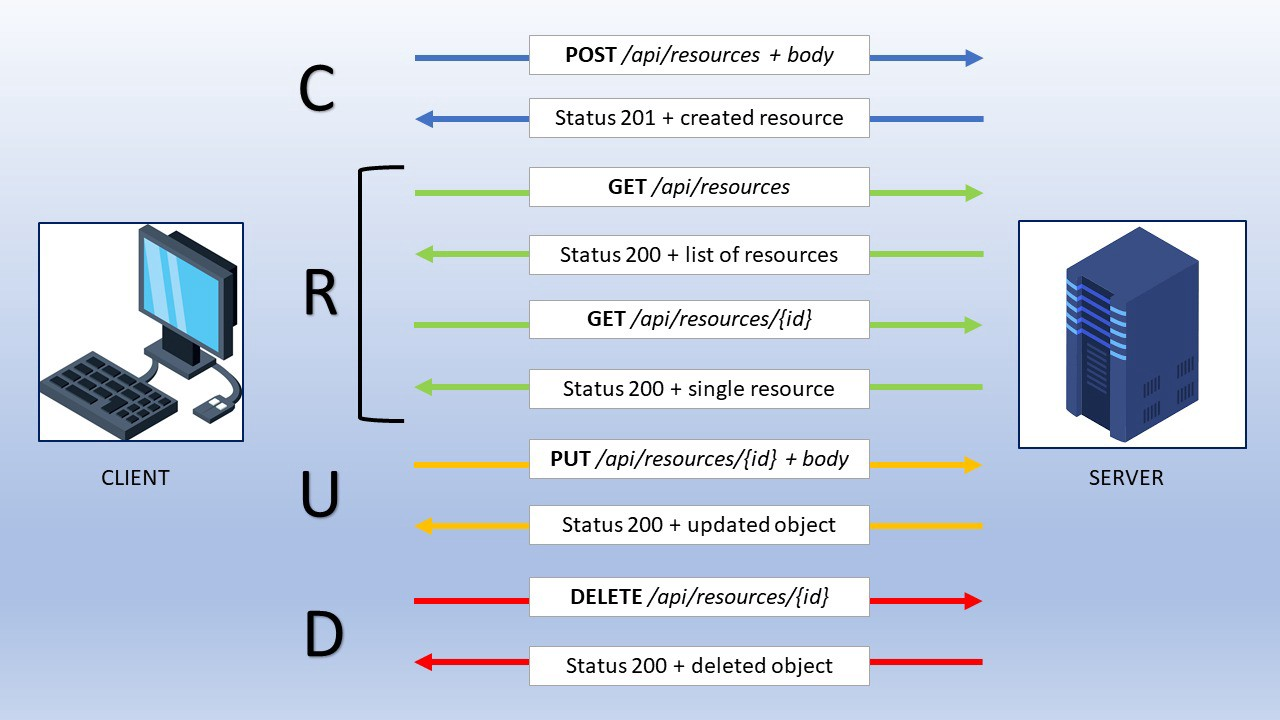
\includegraphics[width=\textwidth]{Figures/1. Tutorial/crud_guidelines.jpeg}
    \captionof{figure}{Princípios CRUD}
    \label{fig: crud guidelines}
\end{figure}

No diagrama acima é possível visualizar como as várias rotas devem ser estruturados para todas as operações (Criar, Ler, Atualizar, e Apagar) e o que cada um deles deverá retornar. De acordo com estes princípios, vamos separar as nossas rotas em dois ficheiros, um para especificar as rotas e o outro para definir o seu comportamento, isto é, as funções que irão fazer as operações reais e devolver a resposta certa a partir das rotas.

\subsubsection{Definindo as Rotas (Endpoints)}

Dentro da nossa pasta \texttt{src}, vamos agora criar uma nova pasta \texttt{routes}, com um ficheiro \texttt{products.routes.js} dentro. No terminal, vamos escrever o seguinte:

\lstinputlisting[language=SH, caption=Comandos para criar as rotas]{Listings/1. Tutorial/create_routes.sh}

Neste ficheiro iremos exportar uma função que leva três parâmetro: a aplicação Fastify, e devolve uma lista de rotas a serem adicionadas à aplicação. Especificamos o verbo HTTP a ser tratado, um URL, e, finalmente, uma função \textit{handler}, que iremos construir numa fase posterior, para cada rota.

\lstinputlisting[language=ES6, caption=Ficheiro models/products.routes.js]{Listings/1. Tutorial/routes_products_1.js}

Com estas rotas, somos agora capazes de realizar uma chamada HTTP do tipo:

\begin{itemize}
    \item \textbf{POST} à rota \texttt{api/products} para Criar um produto
    \item \textbf{GET} à rota \texttt{api/products} para obter uma Lista de todos os produtos
    \item \textbf{GET} à rota \texttt{api/products/:id} para Obter os detalhes de um dado produto
    \item \textbf{PATCH} à rota \texttt{api/products/:id} para Atualizar um dado produto
    \item \textbf{DELETE} à rota \texttt{api/products/:id} para Apagar um dado produto
\end{itemize}

O \texttt{:id} é um \textit{placeholder} para o identificador do nosso documento, permitindo-nos assim aceder ao mesmo através dos parâmetros de entrada do nosso pedido HTTP, na prática utilizando \texttt{request.params.id}.

Vale notar que por pré-definição o Fastify aceita apenas JSON (\texttt{application/json}) como tipo de entrada para o \texttt{body}. É possível adicionar suporte ao tipo de dados de um formulário HTML comum (\texttt{application/x-www-form-urlencoded}) bastando para isso adicionar o \textit{plugin} \textbf{@fastify/formbody} \cite{noauthor_fastifyformbody_nodate}, demonstrado na secção ???. à semelhança do \textbf{Express.js} também é possível suportar o carregamento de ficheiros através do \texttt{multipart/form-data} recorrendo ao \textit{plugin} \textbf{@fastify/multipart} \cite{noauthor_fastifymultipart_nodate}, não abordado neste tutorial.

Como visto acima, precisamos de acesso ao objeto da aplicação fastify para executar os manipuladores das rotas sobre ele, por isso devemos importar este ficheiro para o nosso \texttt{src/index.js} e chamá-lo com o app fastify como seu parâmetro. O Fastify permite-nos registar rotas através da função \texttt{app.register()} e definir prefixos para as mesmas, o que poderemos utilizar para simplificar a nomeação das nossas rotas e evitar erros. Deste modo, começamos por definir um roteador geral para a aplicação com o prefixo \texttt{"/api"} e dentro dele registamos um novo roteador para os nossos produtos que fará uso do nosso ficheiro de rotas e terá o prefixo \texttt{"/products"}. Resultado das alterações ao ficheiro \texttt{src/index.js} em seguida:

\lstinputlisting[language=ES6, caption=Ficheiro index.js atualizado com as rotas]{Listings/1. Tutorial/index_2.js}

\subsubsection{Definindo os Controladoras (Handlers)}

Depois de termos definido as nossas rotas, teremos de definir \textit{handlers} para cada uma delas. Por uma questão de simplicidade deslocaremos as nossas funções de manipulação para um ficheiro externo, onde criaremos a lógica necessária e a exportaremos e as designaremos para as suas respetivas rotas. Estes ficheiros são referidos como controladores. Como primeiro passo, estabelecer uma pasta de controladores no nosso diretório \texttt{src} e adicionar um novo ficheiro intitulado \texttt{products.controller.js}. Vamos abrir o nosso terminal dentro da pasta raiz do projeto e escrever:

\lstinputlisting[language=SH, caption=Comandos para criar os controladores]{Listings/1. Tutorial/create_controllers.sh}

Vamos agora trabalhar no novo controlador:

\lstinputlisting[language=ES6, caption=Ficheiro controllers/products.controller.js]{Listings/1. Tutorial/controller_products_1.js}

Antes de mais, temos de importar o nosso modelo de Produto, que será utilizado para realizar as transações na base de dados utilizando os métodos do Mongoose. Construímos então uma função para cada operação e marcámos-los como assíncronos, porque a nossa base de dados exigirá algum tempo para completar o seu processamento e não poderemos continuaras nossas operações enquanto tais pedidos não forem concluídos.

Vamos colocar a implementação dos \textit{handlers} em espera por agora e apenas conectar o nosso ficheiro de rotas a estas funções recentemente declaradas. Importamos o controlador e atribuímos as funções apropriadas dentro do ficheiro \texttt{products.routes.js}:

\lstinputlisting[language=ES6, caption=Ficheiro routes/products.routes.js atualizado com o controlador]{Listings/1. Tutorial/routes_products_2.js}

\subsection{Implementar os Controladores}

Vamos agora concentrar-nos em cada uma das nossas funções \textit{handler} dentro do \texttt{products.controller.js}.

\subsubsection{Criar um Produto}

Para criar um produto, devemos primeiro extrair informações do corpo (\texttt{request}) do pedido sobre o novo produto que vamos criar. Em seguida, utilizaremos o método \texttt{create} do Mongoose para criar um novo documento e devolvê-lo. Podemos agora definir o estado HTTP apropriado (201 Created) e devolver o nosso novo produto, de acordo com as convenções REST:

\lstinputlisting[language=ES6, caption=Função para criar um produto]{Listings/1. Tutorial/create_product.js}

\subsubsection{Obter a Lista de Proputos}

Esta é provavelmente a função mais simples. Receberemos o nosso pedido GET e executaremos a função de pesquisa no nosso modelo Product, passando um objeto vazio como parâmetro. O primeiro parâmetro é um objeto de consulta do MongoDB que especifica quais os produtos a obter com base em determinados critérios. Como resultado, o objeto vazio devolverá toda a coleção de produtos sem quaisquer restrições. Podemos então retornar os mesmos com o seguinte:

\lstinputlisting[language=ES6, caption=Função para listar os produtos]{Listings/1. Tutorial/list_products.js}

\subsubsection{Obter um Dado Produto}

O primeiro passo desta vez será obter o identificador único do produto que queremos do URL de pedido. Quando incluí-mos \texttt{placeholders} no URL da rota (como fizemos com o \texttt{:id} nas nossas rotas), eles aparecerão no objeto \texttt{request.params}. Após a obtenção do \texttt{id}, podemos utilizar o método \texttt{findById()} no modelo Product para recuperar o produto desejado, fornecendo o \texttt{id} como única parâmetro.

\lstinputlisting[language=ES6, caption=Função para obter um dado produto]{Listings/1. Tutorial/get_product.js}

\subsubsection{Atualizar um Produto}

A atualização implica que extraímos tanto o corpo do pedido como o identificador do produto do URL. As características do produto que necessitam de ser alteradas estarão no \texttt{body}, enquanto o \texttt{id} será utilizado para determinar qual o produto que precisa de ser atualizada. Podemos utilizar o método \texttt{findByIdAndUpdate()} com estas duas informações, fornecendo o \texttt{id} da nota como primeiro argumento e os dados do \texttt{body} como segundo argumento.

Ao contrário dos métodos \texttt{create}, \texttt{find} e \texttt{findById}, \texttt{findByIdAndUpdate} não devolve o objeto alterado por pré-definição, para alterar este comportamento é necessário fornecer um terceiro argumento à mesma, argumento este que deverá ser um objeto que defina a propriedade \texttt{"new"} como verdadeiro, de modo a que possamos responder com a nota recentemente alterada.

\lstinputlisting[language=ES6, caption=Função para atualizar um dado produto]{Listings/1. Tutorial/update_product.js}

\subsubsection{Apagar um Produto}

A eliminação de um produto será o último \texttt{handler} a ser feito. Neste caso não precisamos do \texttt{body}, tudo o que precisamos de fazer é obter o identificador do URL e fornecê-la ao método \texttt{findByIdAndDelete}. Esta função ao ser executada retorna o documento atual antes de eliminar o mesmo, pelo qual basta apenas devolve-lo na nossa resposta:

\lstinputlisting[language=ES6, caption=Função para apagar um dado produto]{Listings/1. Tutorial/delete_product.js}

\subsubsection{Controlador Final}

Pronto! Finaliza-mos o nosso ficheiro do controlador de produtos:

\lstinputlisting[language=ES6, caption=Ficheiro controller/products.controller.js atualizado com os handlers]{Listings/1. Tutorial/controller_products_2.js}

\subsection{Plugin @fastify/formbody}

O Fastify por pré-definição suporta apenas JSON no \texttt{body}. Este \textit{plugin} simples adiciona um \textit{parser} para o tipo de conteúdo \texttt{application/x-www-form-urlencoded}.

Primeiramente precisamos de instalar este plugin como uma dependência do nosso projeto:

\lstinputlisting[language=SH, caption=Comandos para a instalar o plugin @fastify/formbody]{Listings/1. Tutorial/install_formbody.sh}

Em Fastify podemos considerar que um \textit{Middleware} é um \textit{Plugin}, na realidade, à semelhança do JavaScript em que tudo é um objeto, em Fastify tudo é um \textit{plugin}. Para utilizar este \textit{plugin} na aplicação basta registar o mesmo na aplicação fastify:

\lstinputlisting[language=ES6, caption=Ficheiro index.js com @fastify/formbody]{Listings/1. Tutorial/index_3.js}

\newpage

% Creates the conclusion chapter
\section{Conclusão} \label{section: conclusion}

Com este projeto foi possível explorar como utilizar a \textit{framework} fastify para o desenvolvimento de operações CRUD básicas do lado do servidor. Podemos ainda explorar como utilizar plugins/middlewares no fastify, mais concretamente como suportar diferentes \textit{parsers} para o \textit{body}.

Esta aplicação de exemplo, apesar que simples, demonstra o potencial das \textit{frameworks} web e o quanto estas podem ajudar tanto no tempo de desenvolvimento como na qualidade do produto final.

Poderá encontrar todo o código do projeto desenvolvido em \url{https://github.com/IPS-MES-Projects/mes-sii-trabalho-tp/tree/main/Exemplo/api-ementa}.
\newpage

% Creates references using the Biblatex
\printbibliography[heading=bibintoc]
\newpage

\appendix % Any section after this command will have a letter as an index

% Adds an appendix entry
% \input{Chapters/A. Appendix A}
% \newpage

\end{document}
